%************************************************
\chapter{Risultati e discussione}\label{ch:risultati}
%************************************************

% ***********************************************
% [ ] Mettere i grafici con le tre classi
% ***********************************************

Per l'implementazione dell'algoritmo è stato scelto il ben noto 
data set Iris, consistente in una tabella di lunghezze e larghezze 
del petalo e del sepalo collegate a tre specie di fiore Iris. 
Come evidenziato in Schuld et al. \cite{schuld}, 
l'insieme dati si è dovuto standardizzare e 
normalizzare prima dell'utilizzo. 
Il passo successivo è stato ripetere l'esperienza dell'articolo 
per comprenderne appieno il funzionamento e poterlo estendere. 
Questa tesi parte dalla situazione base, in cui
si usano due caratteristiche delle 
quattro disponibili, due vettori di apprendimento 
e si possono classificare solo due classi alla volta. 
Questa versione esemplificativa è stata fatta girare con successo 
sul processore quantistico a 5 qubit messo a disposizione dall'IBM.
Di fronte alla disponibilità di un nuovo computer quantistico a 16 
qubit\footnote{\url{https://developer.ibm.com/dwblog/2017/quantum-computing-16-qubit-processor/}, 
Recuperato l'8 settembre 2019}, 
ci si chiede quali sono le prossibilità di miglioramento delle 
implementazioni pratiche. Si è lavorato sulle seguenti proprietà: 
\begin{itemize}
    \item aumentare il numero di classi riconosciute;
    \item aumentare il numero di caratteristiche considerate;
    \item aumentare il numero di vettori di training.
\end{itemize}
Per fare ciò, si è dovuto tenere in considerazione i compromessi 
in termini di numero di qubit ed efficienza di classificazione: 
infatti, per realizzare ognuno di questi punti c'è bisogno di impegnare 
più qubit, non solo per una questione di memoria, ma anche per 
la complessità delle operazioni da effettuare; un'esempio è dato 
dalla porta $C^n R_y (\theta)$, usata nel procedimento di costruzione 
della \ac{QRAM} (vedi sezione \ref{sec:ff-qram}), che necessita di un 
qubit ancilla in più per ogni qubit di controllo aggiuntivo. 

\section{Ottimizzazione dei dati}

Il data set Iris completo si presenta nella forma mostrata in figura 
\ref{fig:iris_grezzi}, dove sono indicate le prime due caratteristiche 
sugli assi coordinati. 

\begin{figure}[ht]
    \centering
    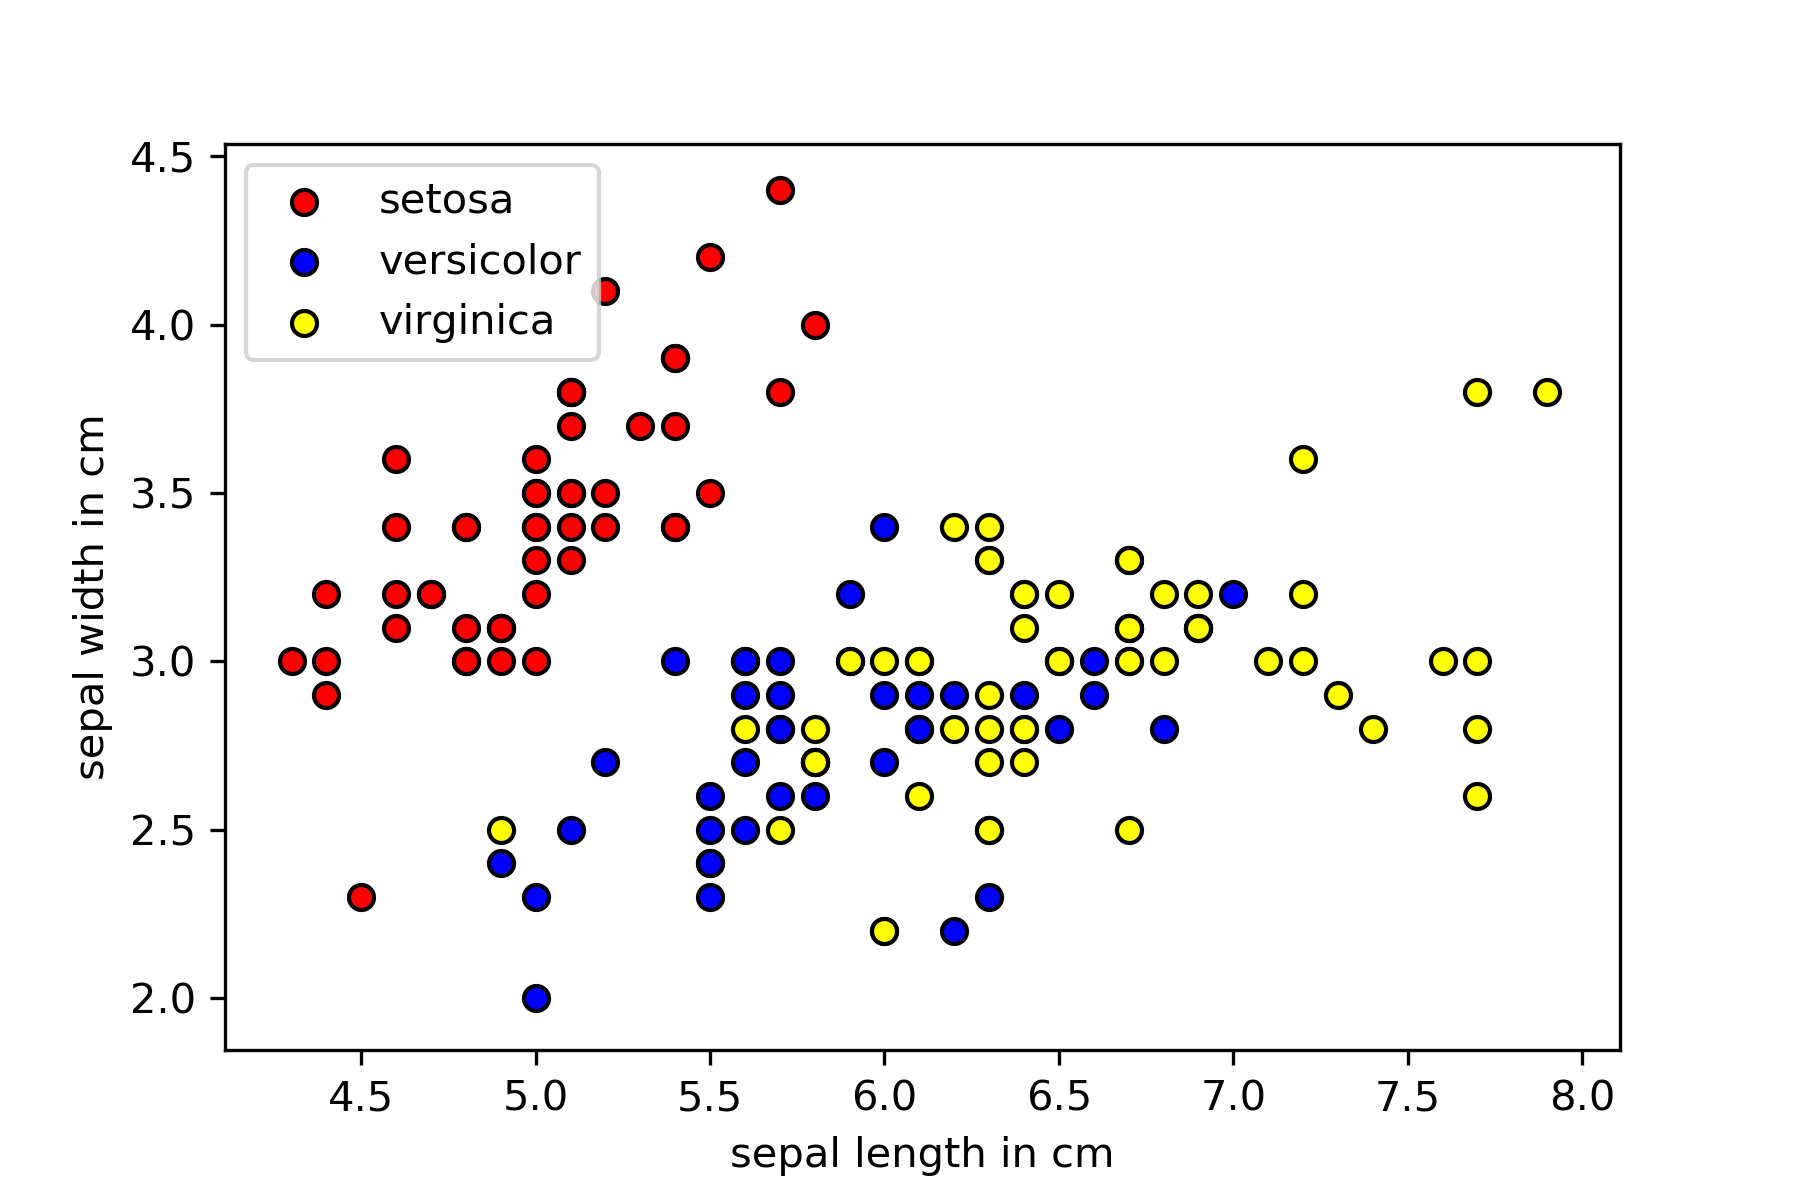
\includegraphics[width=\linewidth]{gfx/iris/irisfeatures}
    \caption{Data set Iris non elaborato}
    \label{fig:iris_grezzi}
\end{figure}

La prima operazione sui dati è la standardizzazione, che trasla e scala 
i punti in modo che abbiamo media nulla e deviazione standard unitaria. 
Si possono notare gli effetti nella figura \ref{fig:iris_standard}, 
osservando i nuovi valori sugli assi. 

\begin{figure}[h!]
    \centering
    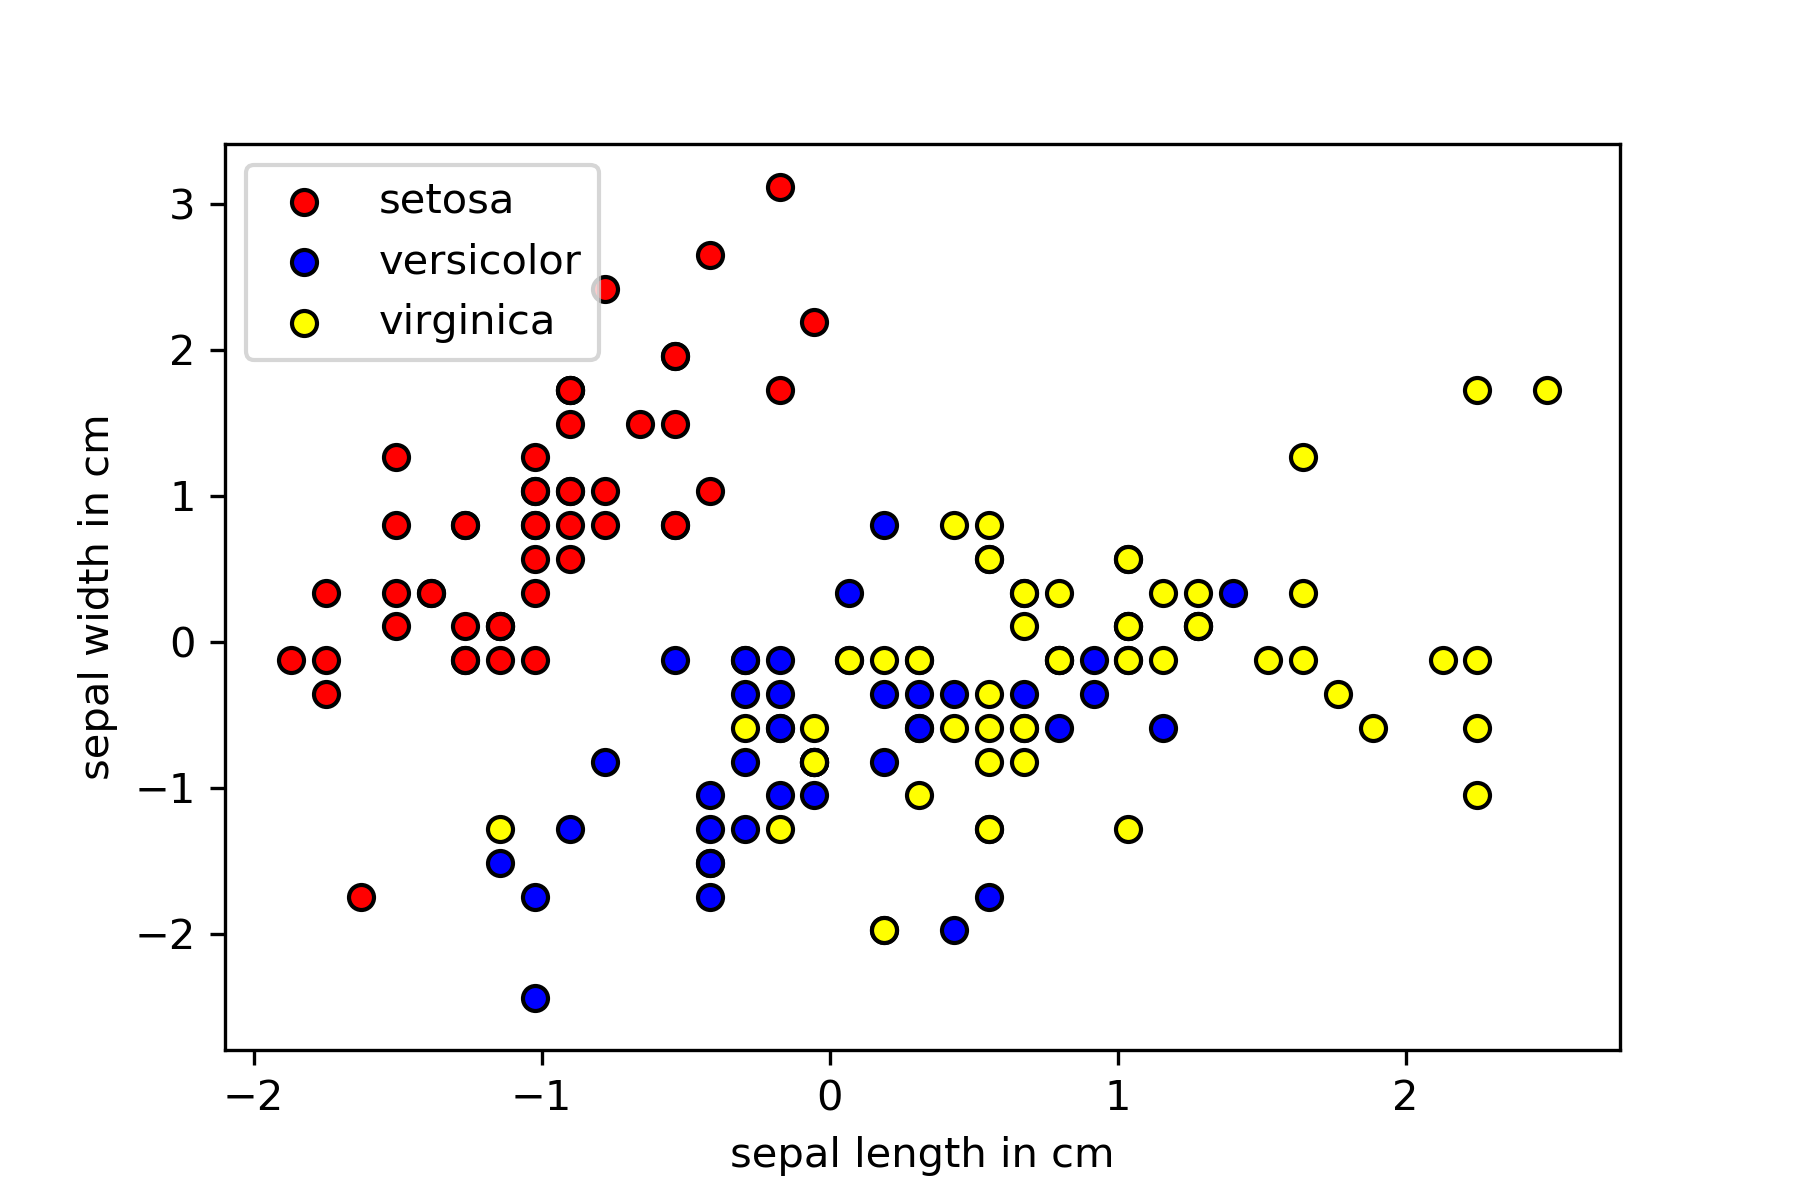
\includegraphics[width=\linewidth]{gfx/iris/irisscaled}
    \caption{Data set Iris standardizzato}
    \label{fig:iris_standard}
\end{figure}

La normalizzazione termina il processo preliminare di ottimizzazione 
dei dati. Si può vedere l'effetto della normalizzazione su un data set 
con due caratteristiche in figura \ref{fig:iris_normal}. 

\begin{figure}[ht]
    \centering
    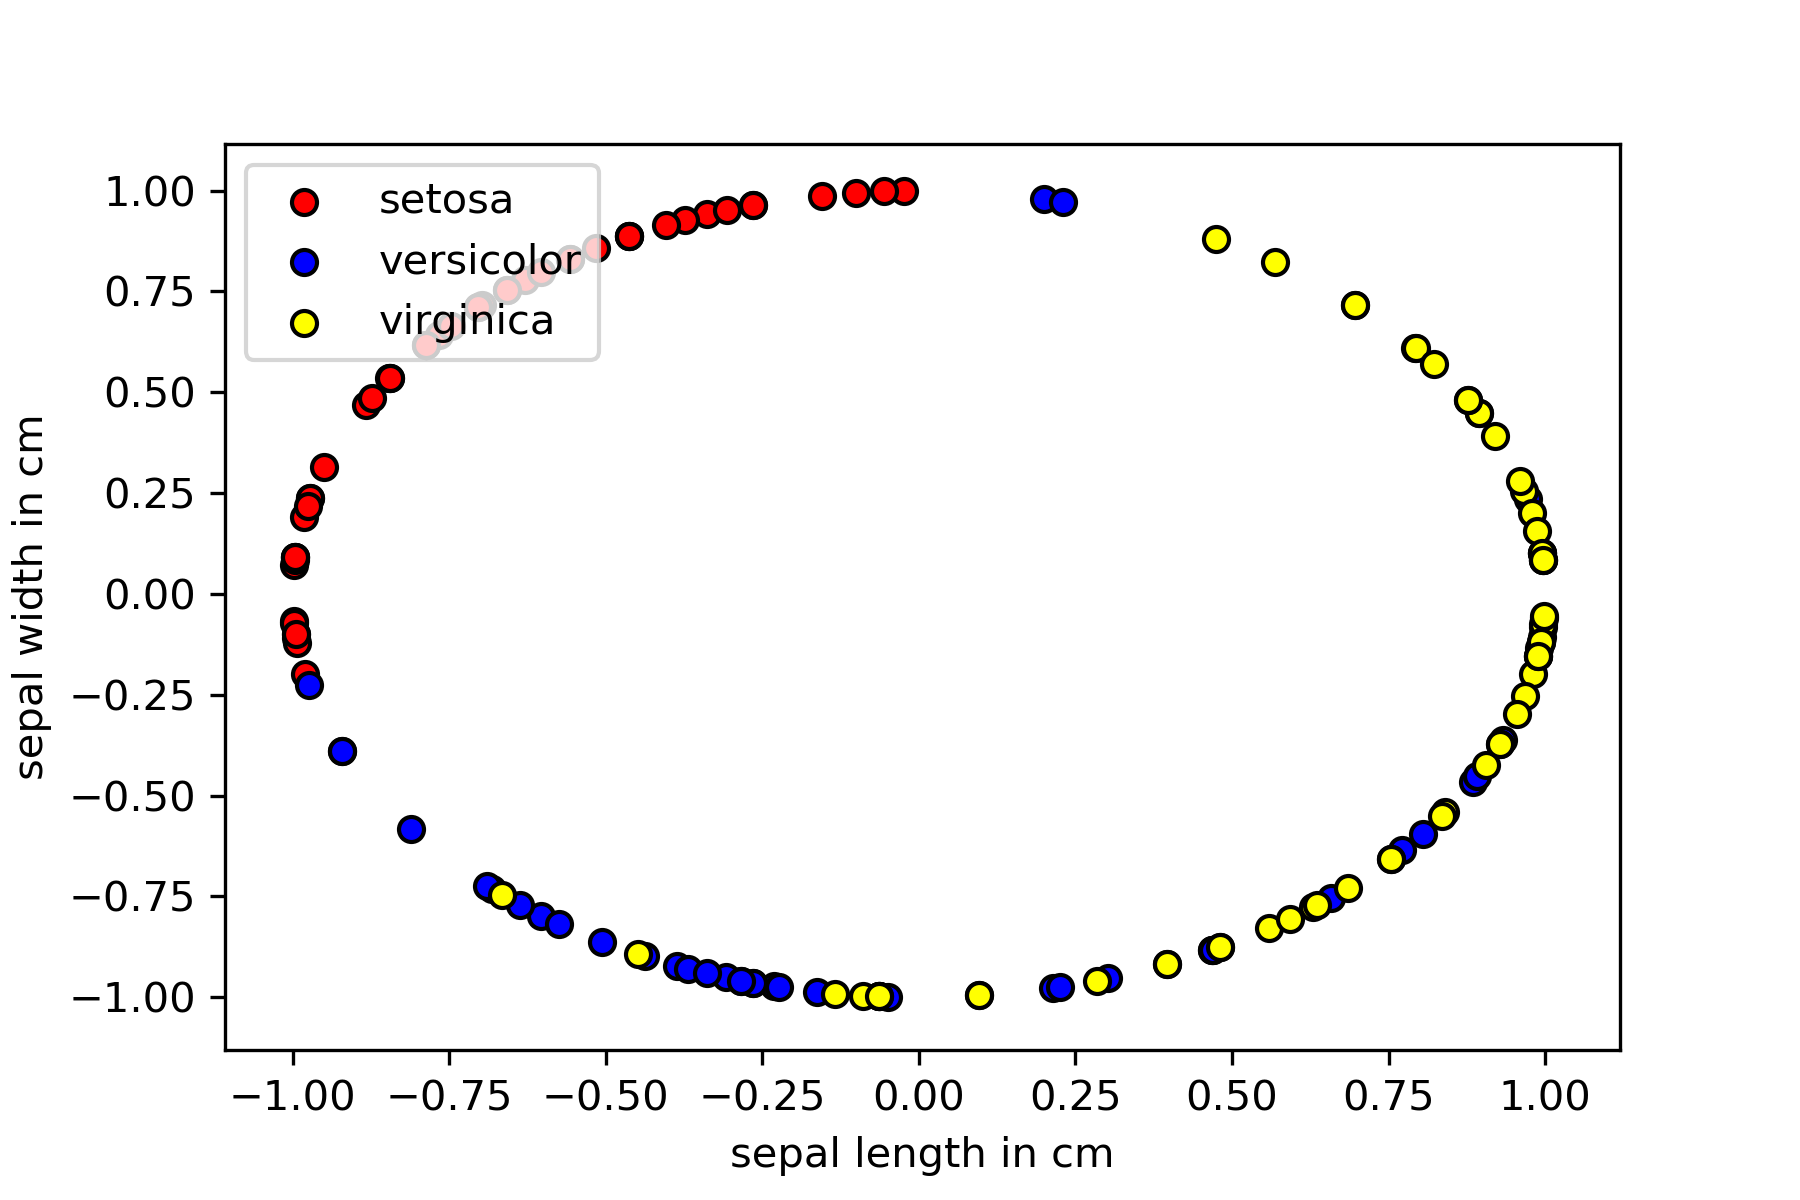
\includegraphics[width=\linewidth]{gfx/iris/irisnormalized}
    \caption{Data set Iris normalizzato}
    \label{fig:iris_normal}
\end{figure}

Avendo effettuato queste operazioni, si deve ora tradurre le coordinate 
di ciascun vettore nello spazio delle caratteristiche in un angolo di rotazione 
da applicare al qubit registro della \ac{QRAM}. 

Facendo riferimento all'eq. \ref{eq:qram.prob}, troviamo che lo stato costruito, 
dopo la misura condizionale, è 
\begin{equation}
    \sum_{l=0}^{M-1} \psi_{\vec{d}^{(l)}}\ket{\vec{d}^{(l)}}\sin\theta^{(l)}\ket{1}_R. 
\end{equation}
La relazione esistente tra i valori $b_l$, ovvero le caratteristiche standardizzate e normalizzate, 
e le ampiezze di probabilità nella \ac{QRAM} è 
\begin{equation}
    \theta^{(l)} = \arcsin b_l. 
\end{equation}

\section{Scrittura dell'algoritmo}

Avendo acquisito le nozioni teoriche e i parametri iniziali, si prova 
adesso a costruire il circuito quantistico attraverso le porte 
dell'insieme universale di base, disponibili grazie all'interfaccia IBM 
Q Experience ed al kit di sviluppo Qiskit. 

Seguendo la figura A.1 in appendice, si 
esamina il circuito quantistico di base: 
\begin{enumerate}
    \item i qubit ancilla ed indice vengono posti in sovrapposizione uniforme; 
    \item il vettore d'input $x$ è posto in entanglement con lo stato fondamentale 
    dell'ancilla;
    \item il vettore di training $t^0$ è posto in entanglement con lo stato eccitato 
    dell'ancilla e con lo stato fondamentale del qubit indice;
    \item il vettore di training $t^1$ è posto in entanglement con lo stato eccitato 
    dell'ancilla e del qubit indice;
    \item il qubit classe è invertito condizionato dal fatto che il qubit indice sia $\ket{1}$; 
    questo completa la preparazione iniziale dello stato; 
    \item nell'ultimo passaggio la porta Hadamard fa interferire le copie di $x$ con i vettori 
    d'apprendimento e l'ancilla è misurata, seguita da una misura del qubit classe. 
\end{enumerate}
Considereremo validi per i nostri scopi solo le misure del qubit classe ottenute quando il 
qubit ancilla è trovato nello stato $\ket{0}$. 
Possiamo notare, tra le altre cose, che la porta $C^n R_y (\theta)$ è in 
realtà formata da una successione di più porte di base. Mentre nei primi tempi 
era necessario inserire manualmente i singoli elementi logici per eseguire una operazione 
complessa, nella realizzazione attuale si è sfruttato il lavoro della comunità 
open source di Qiskit, che ha messo a disposizione comandi veloci per aggiungere 
facilmente porte multi controllate. 

\subsection{Classificazione iniziale}

Si mostra un esempio di risultato di classificazione usando le prime due caratteristiche 
del data set e gli elementi appartenenti alle classi setosa e versicolor. 
Si scelgono come vettori di training un elemento per ciascuna classe, nel nostro caso 
il vettore 34 ed il vettore 86 dal data set, rispettivamente setosa e versicolor. 
Si assegna alla classe setosa lo stato $\ket{0}$ del qubit classe ed alla classe 
versicolor lo stato $\ket{1}$. 
Si sottopongono poi a classificazione, in due esperimenti separati, due vettori sconosciuti: 
il vettore 29 (setosa) ed il vettore 57 (versicolor). 

Il primo passo è simulare l'esperimento sul computer in uso, dato che il problema in esame
è facilmente eseguibile su un comune portatile. I risultati non filtrati per i due esperimenti 
sono visibili nel riquadro \ref{fig:simulazione_circuito}. Nella didascalia sono scritti i conteggi corrispondenti ad un 
determinato esito di misura sui due qubit ancilla e classe. La cifra sulla destra contiene la 
misura del qubit ancilla, quella sulla sinistra del qubit classe. Tali valori, normalizzati ad uno, 
sono rappresentati in un istogramma, che approssima la distribuzione di probabilità degli esiti di 
misura per grandi numeri di esecuzioni dell'algoritmo. Per questo motivo si userà preferibilmente 
un numero di esecuzioni pari al massimo permesso sui computer quantistici dell'IBM, ovvero 8192. 
\begin{figure}[h!]
    \myfloatalign
    \subfloat[Iris setosa] {
        \label{fig:misura_setosa}
        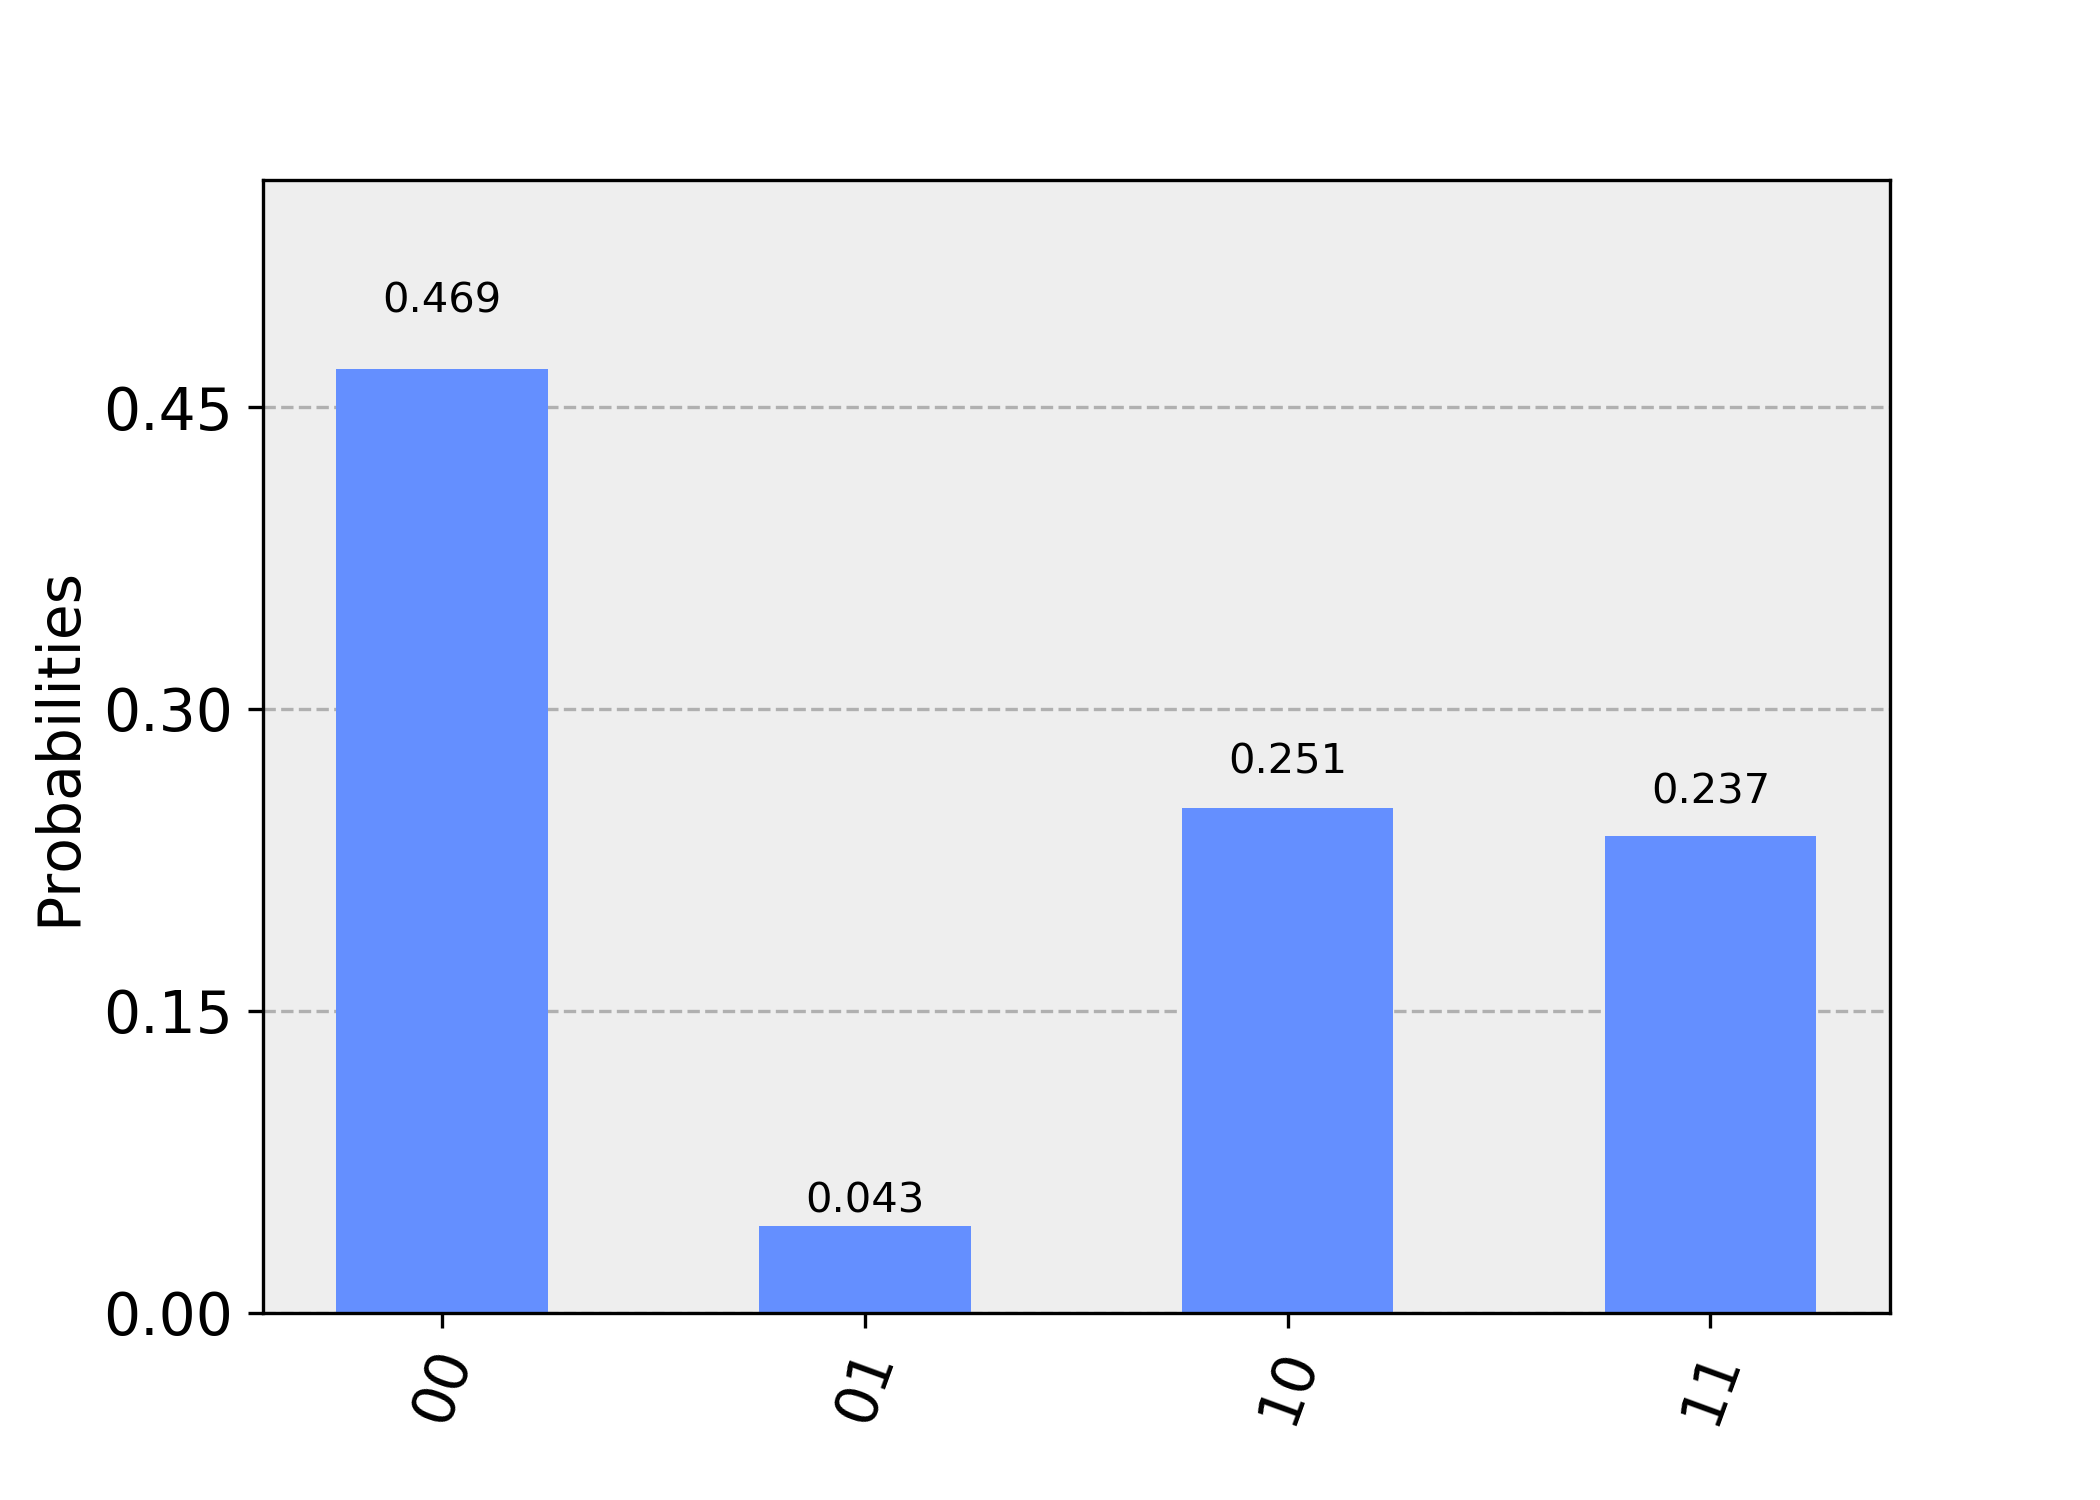
\includegraphics[width=\linewidth]{gfx/misura_setosa}
    } \\
    \subfloat[Iris versicolor] {
        \label{fig:misura_versicolor}
        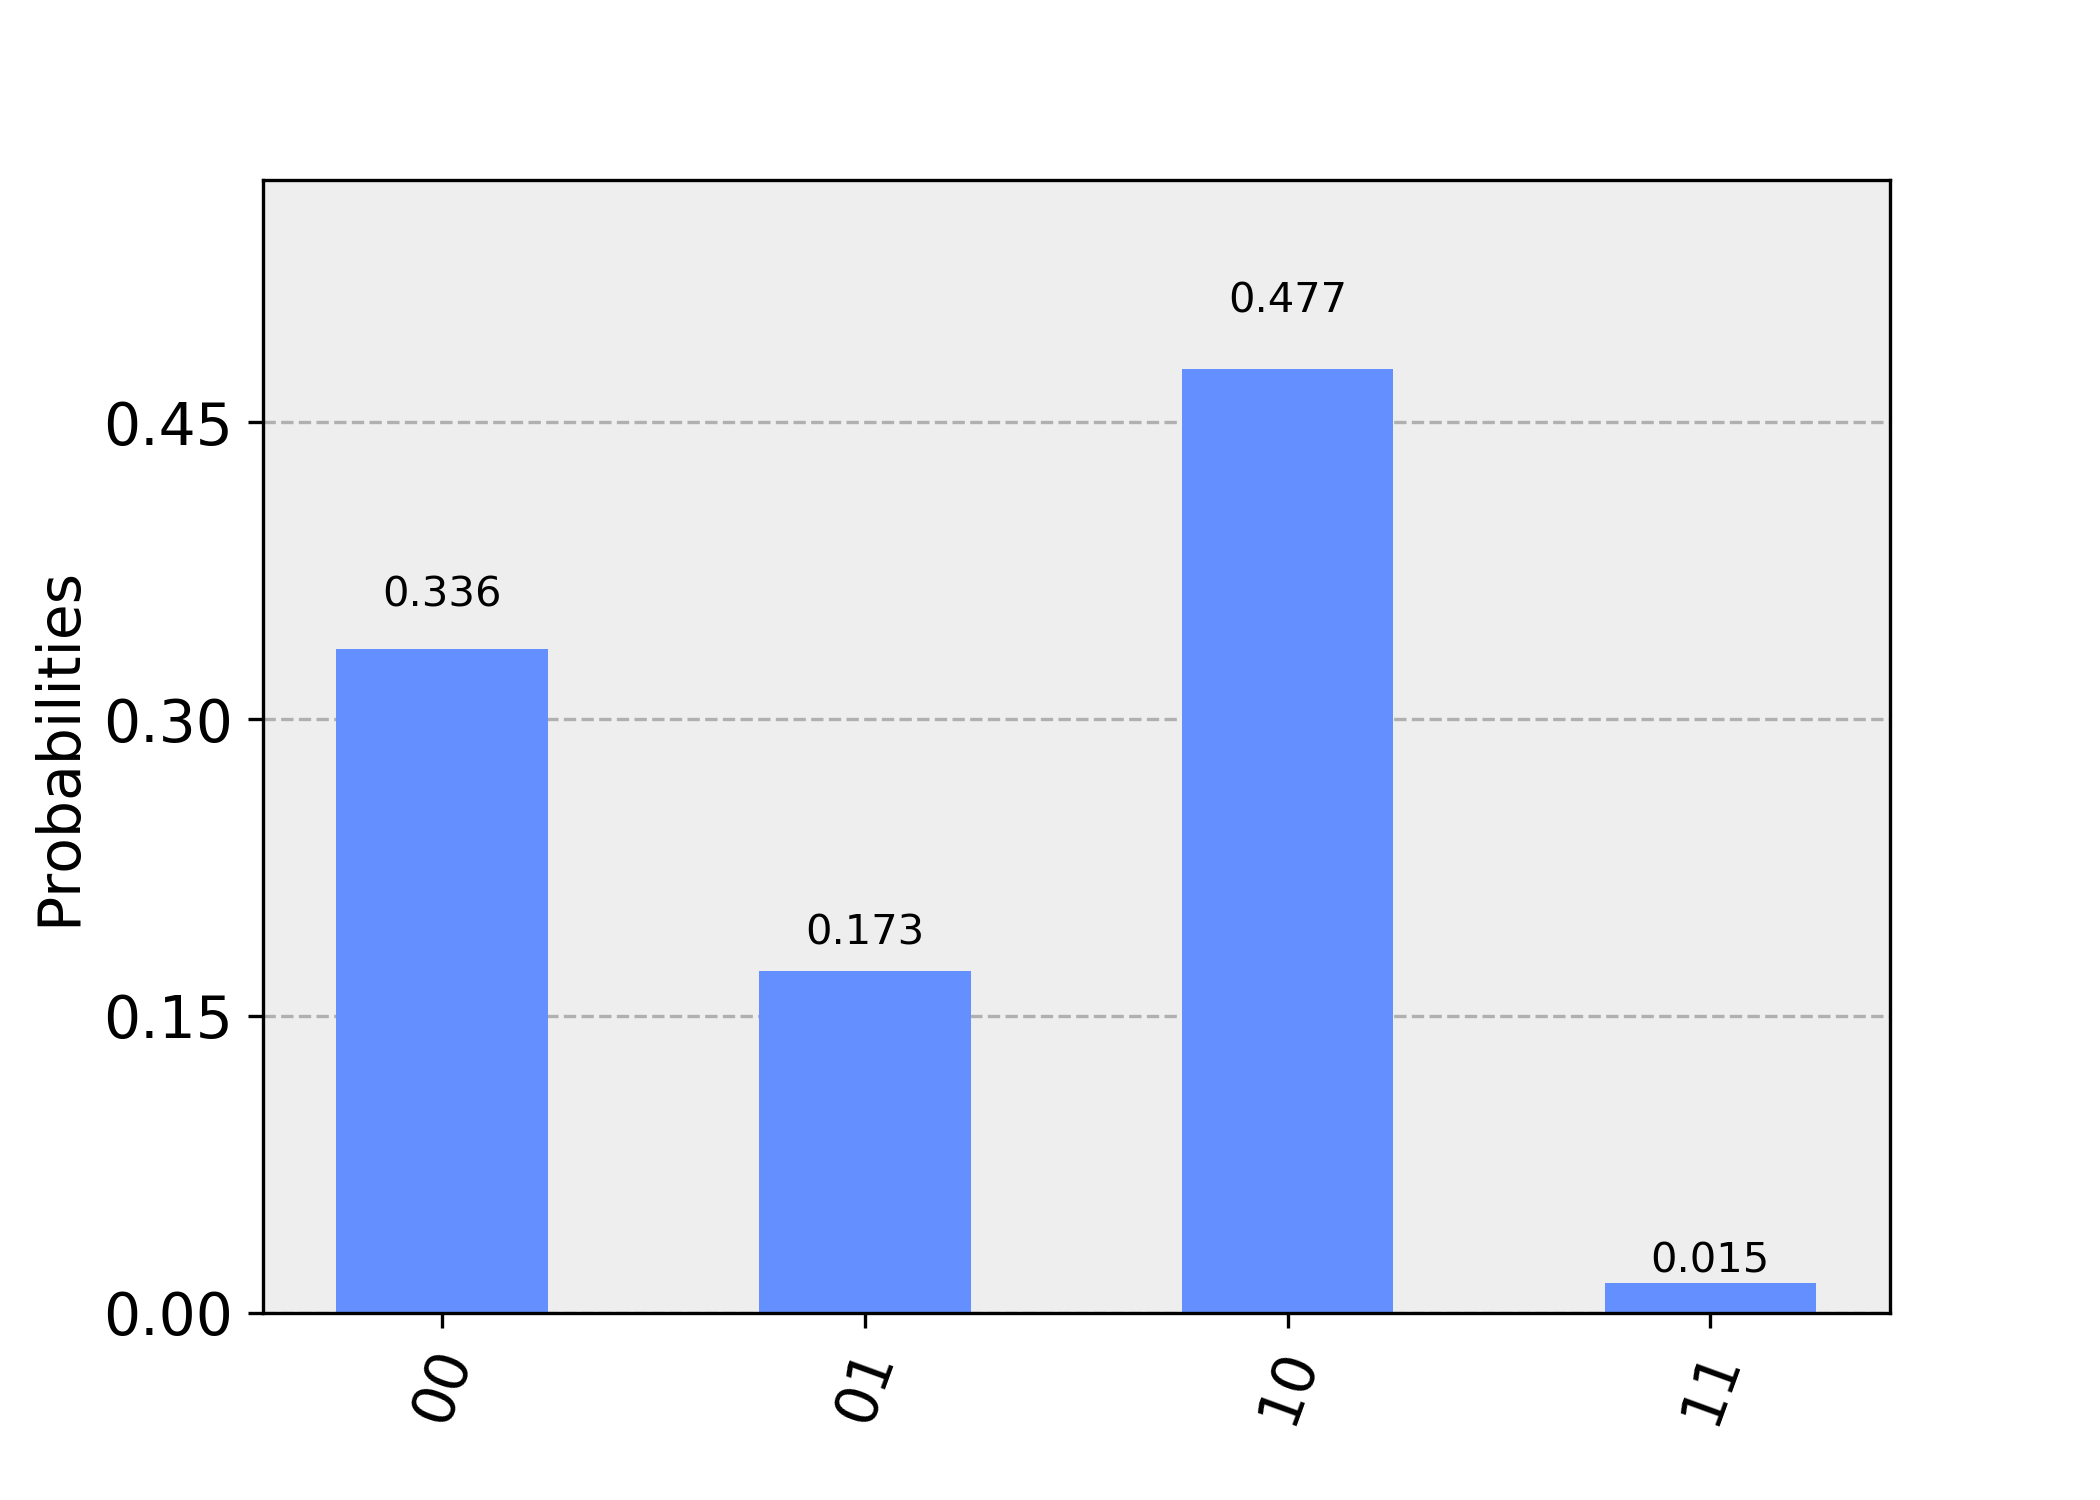
\includegraphics[width=\linewidth]{gfx/misura_versicolor}
    }
    \caption[Simulazione del circuito]%
    {Simulazione del circuito. \par \small 
    I conteggi totali sono: \\
    per setosa \{'00': 3843, '10': 2056, '01': 352, '11': 1941\}; \\
    per versicolor \{'00': 2749, '10': 3908, '01': 1414, '11': 121\}.}
    \label{fig:simulazione_circuito}
\end{figure}
Selezionando i risultati laddove il bit di destra è 0, abbiamo praticamente effettuato 
la misura condizionale necessaria al funzionamento dell'algoritmo. 
Nel riquadro \ref{fig:simulazione_filtrati} sono presentati 
i risultati filtrati in modo da considerare solo i risultati in cui il bit 
ancilla è 0. 
\begin{figure}[h!]
    \myfloatalign
    \subfloat[Iris setosa]{
        \label{fig:misura_setosa_filtrata}
        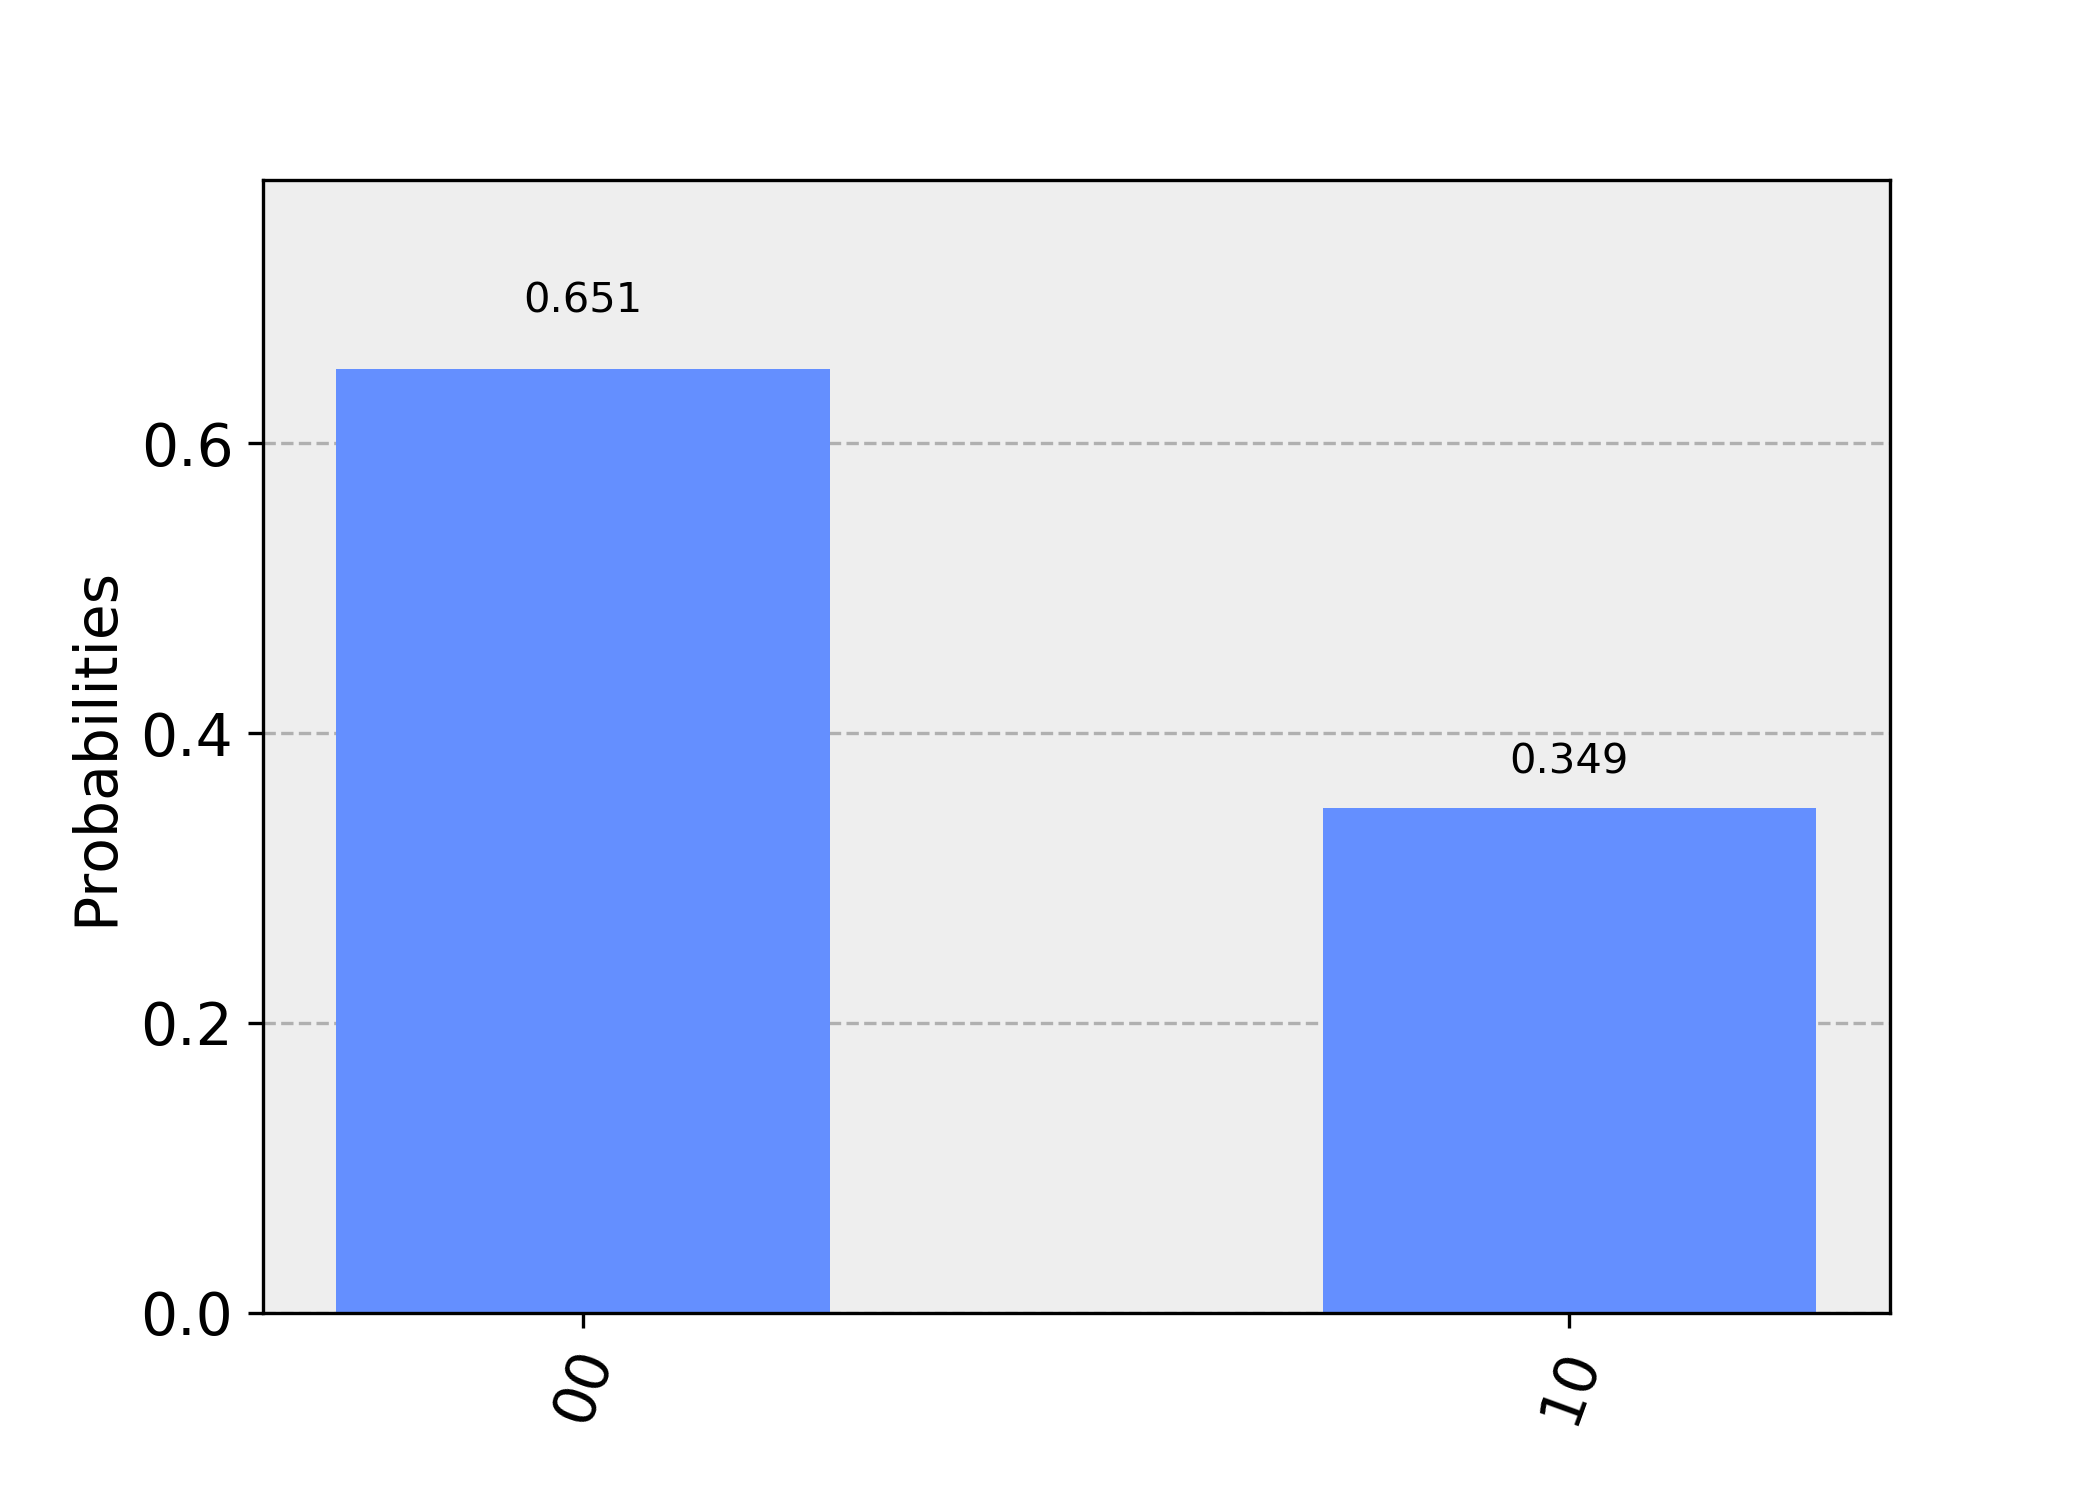
\includegraphics[width=\linewidth]{gfx/misura_setosa_filtrata}
    } \\
    \subfloat[Iris versicolor]{
        \label{fig:misura_versicolor_filtrata}
        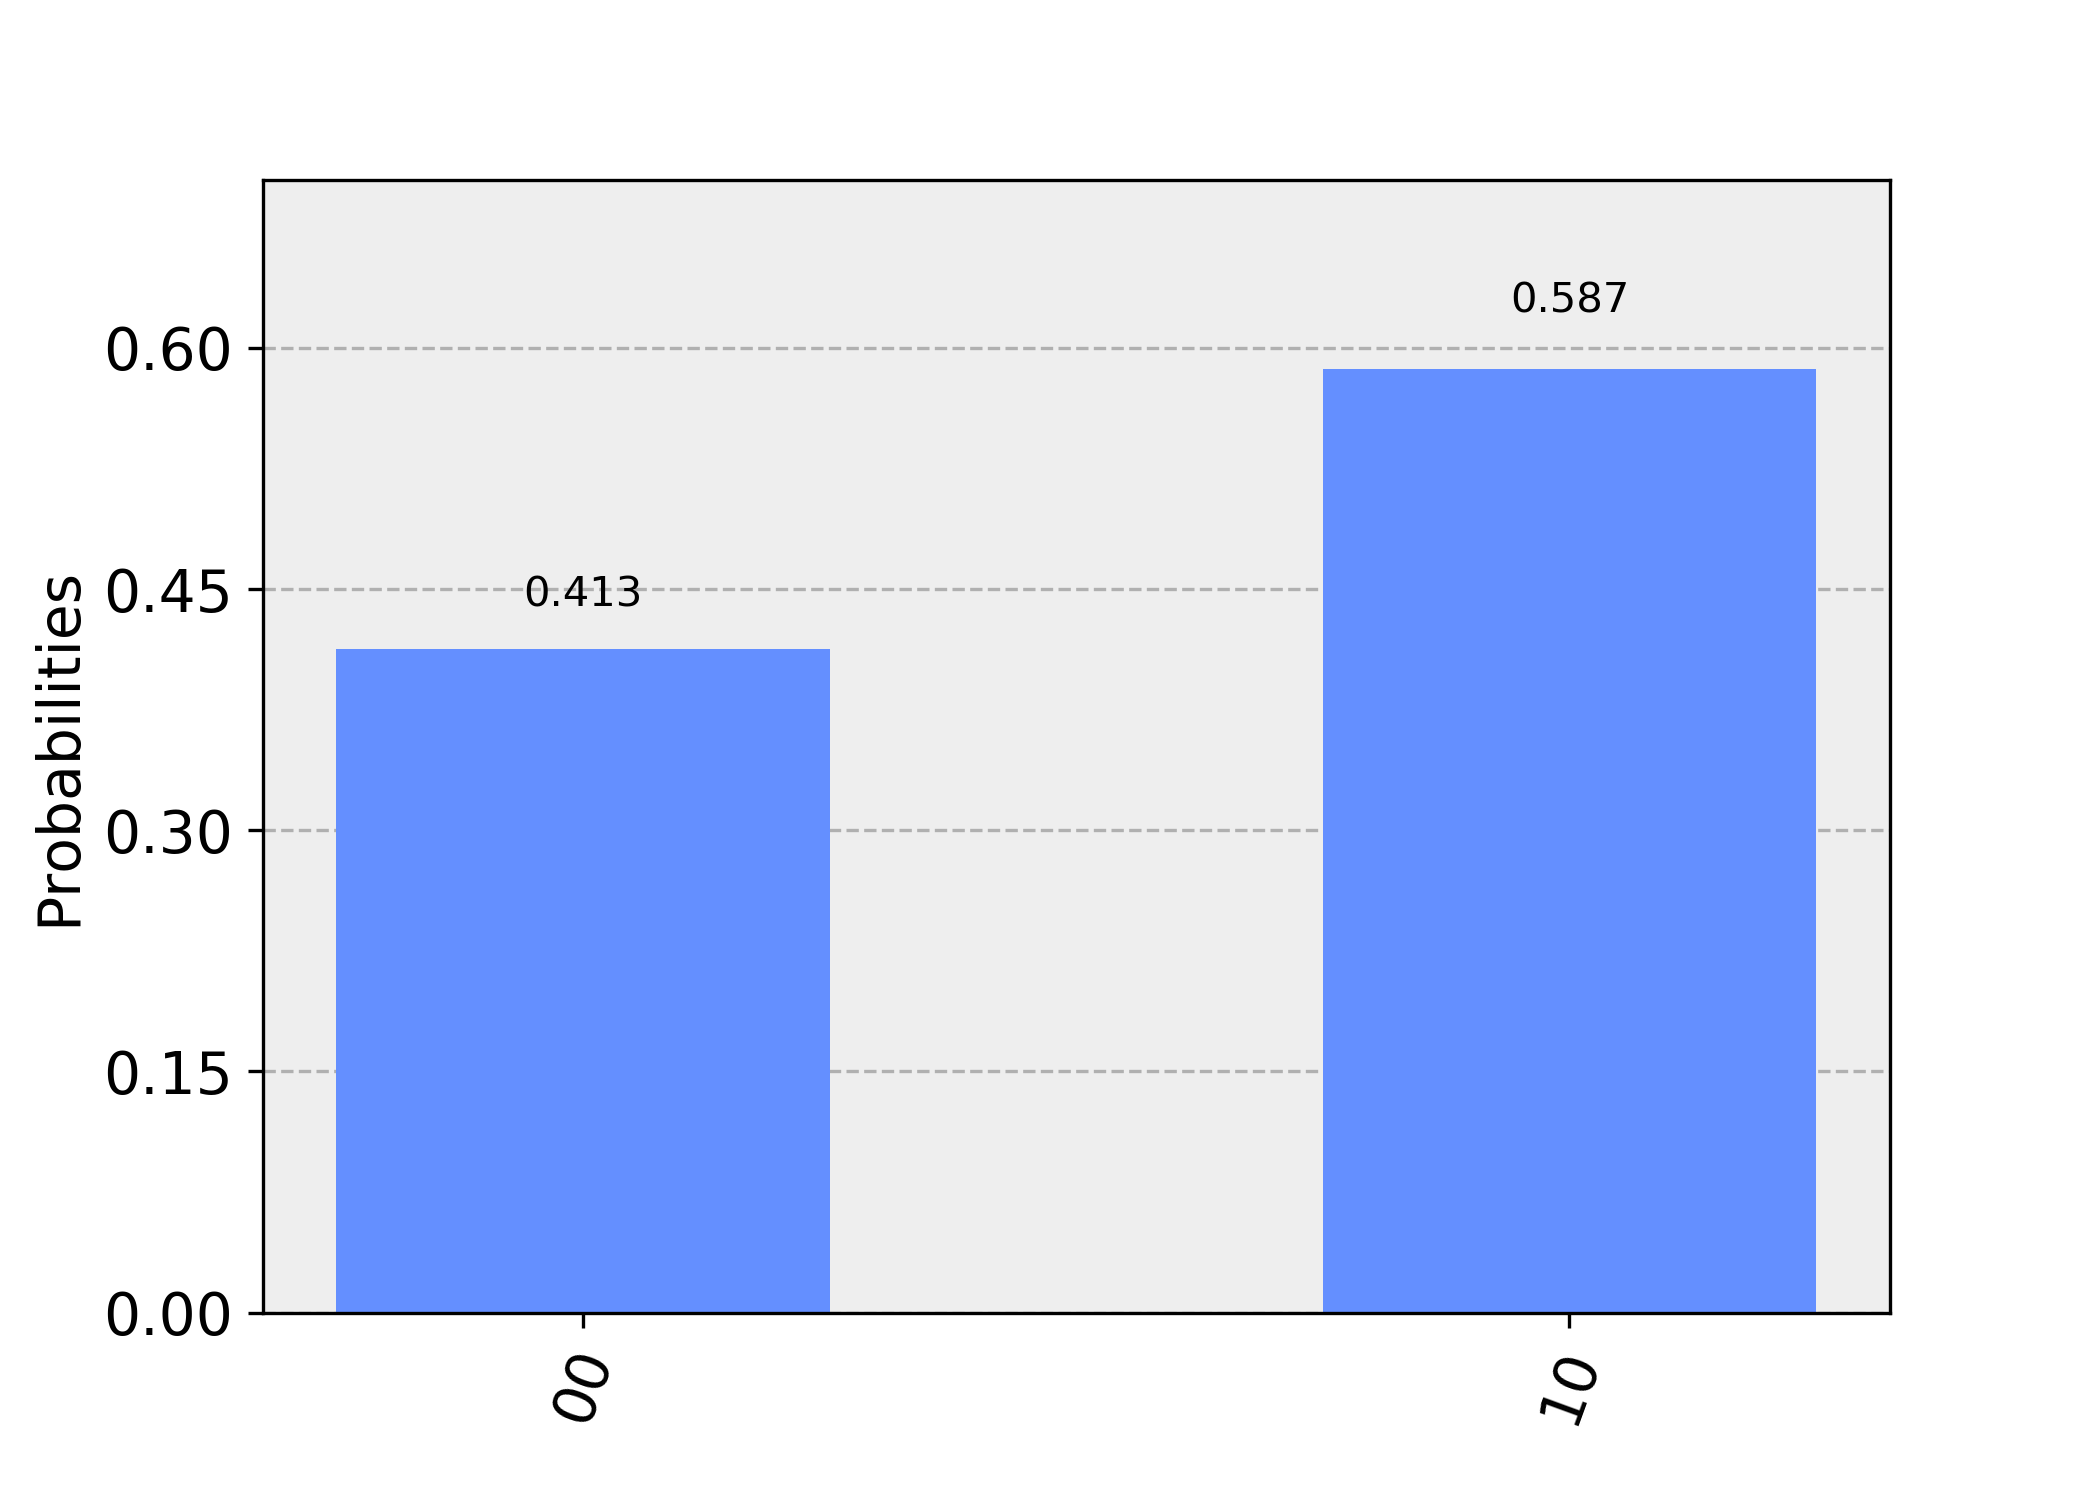
\includegraphics[width=\linewidth]{gfx/misura_versicolor_filtrata}
    }
    \caption{Simulazione del circuito, risultati filtrati}
    \label{fig:simulazione_filtrati}
\end{figure}

Il passo successivo è eseguire questi stessi circuiti quantistici su un vero computer quantistico. 
È stata scelta la macchina a 16 qubit ibmq\_16\_melbourne per ottenere le misure per il 
vettore d'input setosa illustrate in figura \ref{fig:sperimentale_setosa}. 
\begin{figure}[h!]
    \centering
    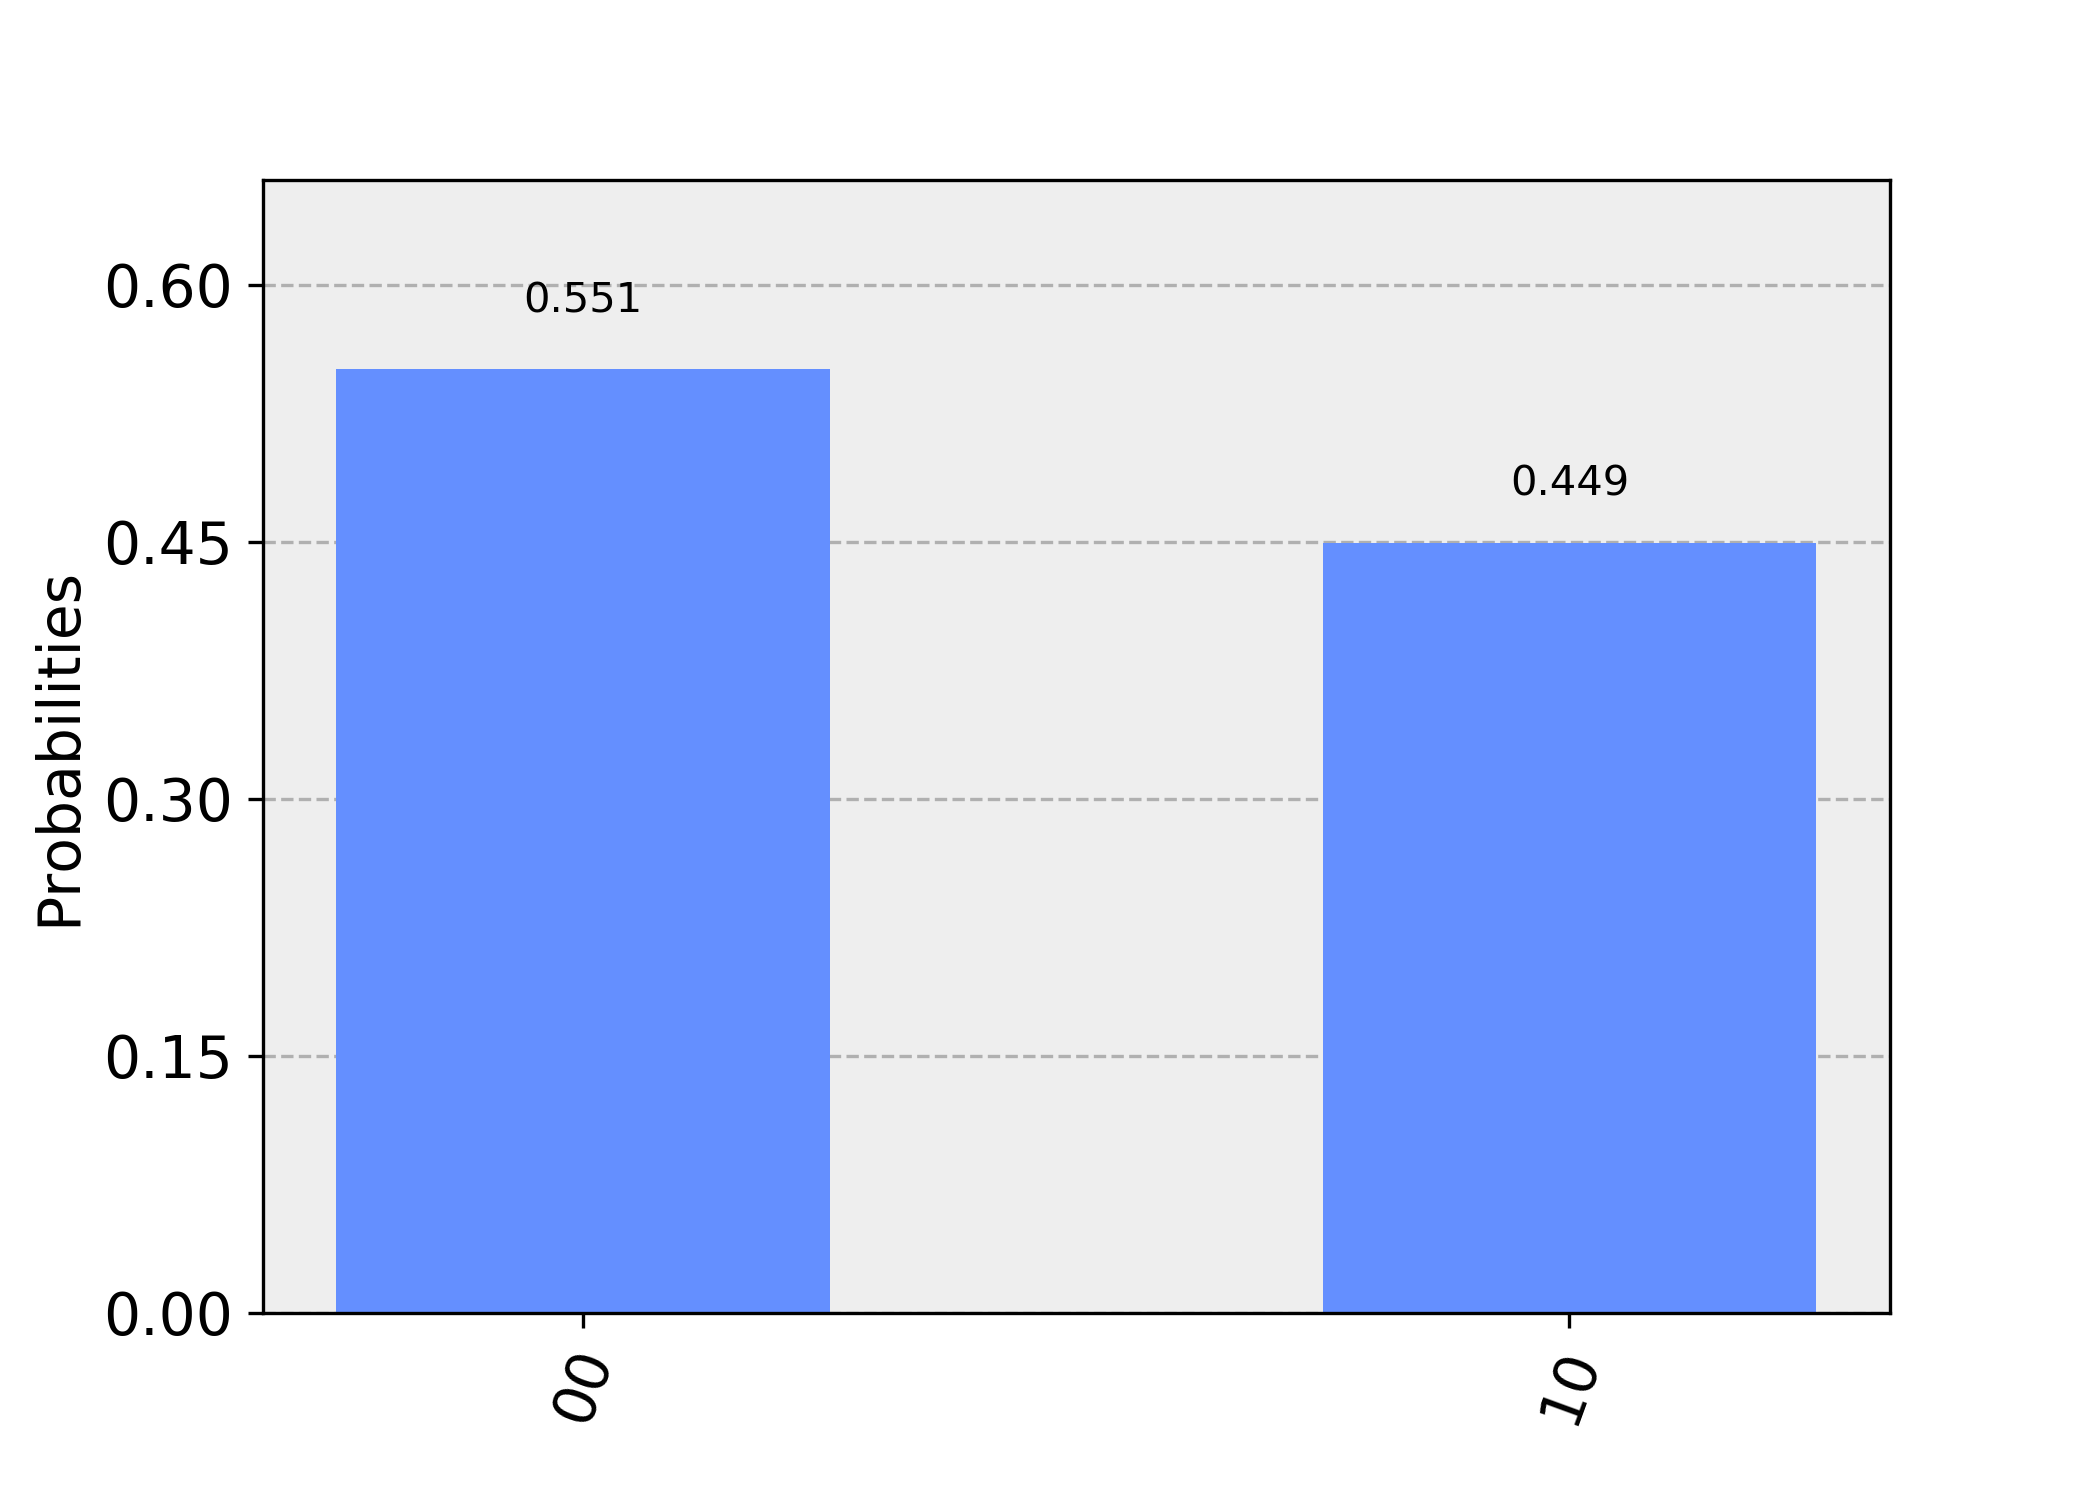
\includegraphics[width=\linewidth]{gfx/misura_setosa_sperimentale}
    \caption{Esecuzione su hardware reale (setosa)}
    \label{fig:sperimentale_setosa}
\end{figure}
Gli inevitabili fenomeni di rumore rendono i risultati meno piccati ma comunque 
distinguibili in questo caso. 

Il discorso è diverso per il confronto tra le classi versicolor e 
virginica: visto che gli elementi di queste due classi non sono linearmente separabili, 
algoritmi come quello qui usato non sono efficaci nella loro distinzione. 
Uno dei metodi per aggirare questo problema è l'uso di feature map \cite{schuld} nel processo 
di ottimizzazione. Infatti le misure effettuate danno risultati erronei o 
ambigui nella maggioranza dei casi (probabilità del 50\% per entrambi i risultati). 

Ad ogni modo, si procederà nel realizzare i punti definiti all'inizio di 
questo capitolo. Condizione necessaria per distinguere le tre classi con un 
solo esperimento è che si possano memorizzare almeno tre vettori di training, 
uno per ciascuna classe. 

\subsection{Aumento del numero di vettori d'apprendimento}

Il numero di stati posseduti da $n$ qubit, come abbiamo visto nella 
sezione sui fondamenti teorici, è $2^n$. Nell'esperimento visto poco 
prima, si è dedicato un solo qubit per segnare l'indice dei vettori di 
apprendimento $\ket{m}$. Aggiungendo ulteriori qubit all'indice possiamo 
immagazzinare successivamente 4, 8, 16, 32, 64, \ldots vettori di training. 
Con 8 qubit per il registro $\ket{m}$ già siamo in grado di immagazzinare 
tutti i vettori del data set Iris. Nel caso di grandi insiemi, tuttavia, 
potrebbe essere appropriato ridurre il numero di vettori di training durante 
il processo di ottimizzazione, adottando un criterio di selezione che includa 
solo i vettori più significativi ai fini della classificazione. 

La spesa totale in termini di risorse coinvolge due qubit per ogni incremento 
che facciamo: infatti, per mettere in entanglement un qubit in più del registro 
$\ket{m}$ con il qubit registro della \ac{QRAM}, abbiamo bisogno di un qubit 
ancilla aggiuntivo per l'operazione $C^n R_y (\theta)$; questi qubit ancilla non 
sono rappresentati nei disegni dei circuiti per semplice convenienza visiva, ma 
se ne può trovare traccia nei frammenti di codice scritti per questa tesi\footnote{Si veda 
\url{https://github.com/visika/Tesi}}.

\subsection{Implementazione multiclasse}

L'aggiunta della capacità di riconoscere tutte le tre classi in una sola esecuzione 
non è di natura differente dall'aggiungere qubit per avere maggiori vettori 
di apprendimento. Passiamo dall'avere un solo qubit classe, che ha associato il 
proprio stato $\ket{0}$ alla prima classe e lo stato $\ket{1}$ alla seconda, 
ad avere due qubit classe ed associare lo stato $\ket{00}$ alla prima classe, 
lo stato $\ket{01}$ alla seconda classe e lo stato $\ket{10}$ alla terza classe. 
Lo stato $\ket{11}$ non è associato ad alcuna classe. 
Nel processo di costruzione dello stato iniziale nella \ac{QRAM}, 
oltre che ai qubit indice, i vettori di addestramento saranno in entanglement 
anche con i relativi stati dei due qubit classe. Osservando la figura \ref{fig:qram_classi} 
si vede che le porte $\overline{c}X$ sui qubit classe sono applicate solo all'inizio e 
alla fine del processo di codifica di tutte le componenti di un vettore di training. 
\begin{figure}[h!]
    \centering
    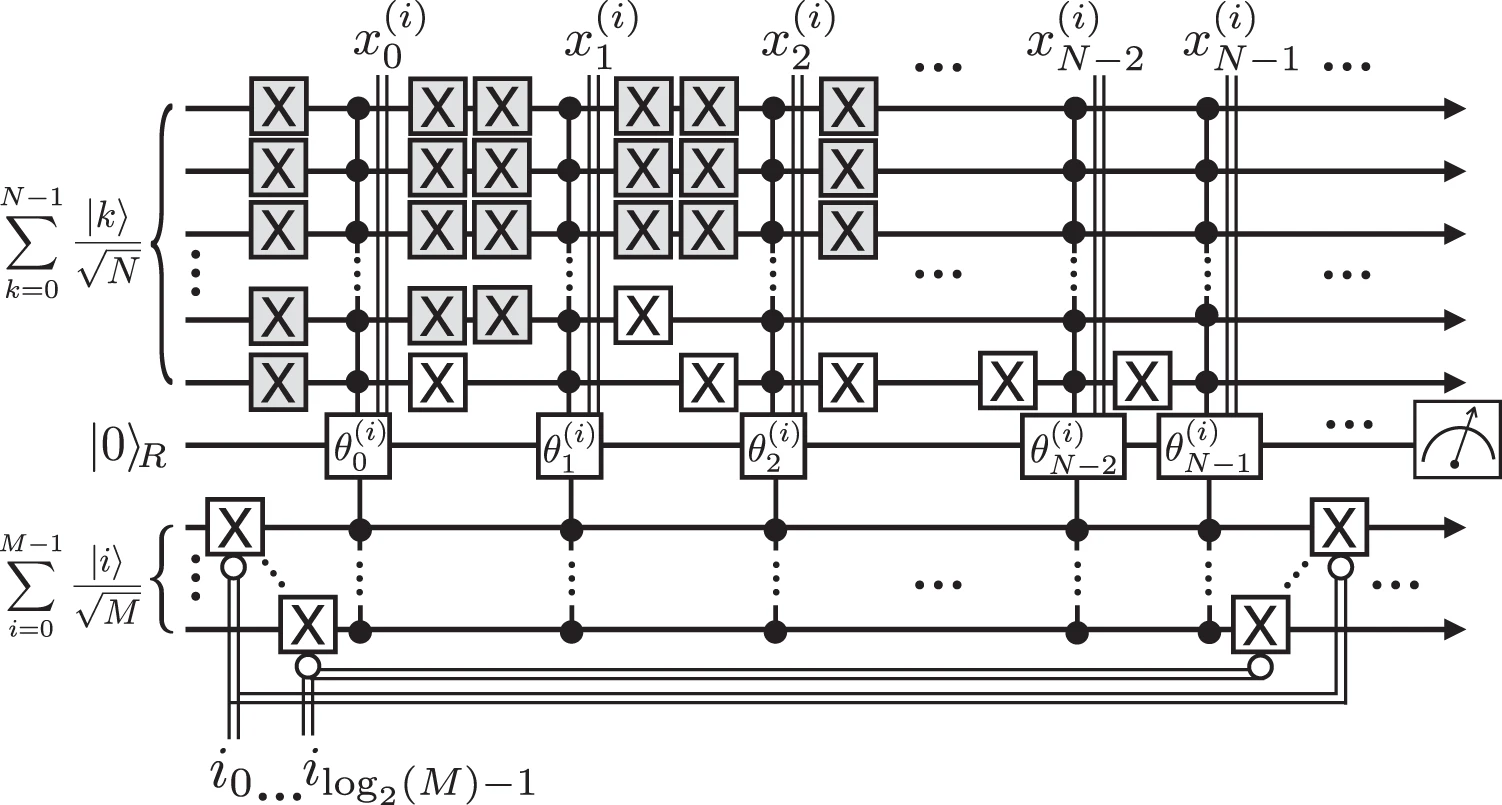
\includegraphics[width=\linewidth]{gfx/qram_classi}
    \caption[Circuito quantistico per preparare il \acs{QDB} per un quantum support vector machine]%
    {Circuito quantistico per preparare il \acs{QDB} per un quantum support vector machine. \par \small 
    Sono mostrate le porte per scrivere solo l'$i$-esimo vettore di apprendimento. Le porte ombreggiate 
    in grigio sono aggiunte esclusivamente per illustrare il processo flip-flop, e non sono implementate 
    in pratica.}
    \label{fig:qram_classi}
\end{figure}

\subsection{Aumento del numero di caratteristiche}

% *********************************************
% Questa parte va aggiustata
% *********************************************

L'Iris data set possiede 4 caratteristiche. È poco dispendioso includerle tutte 
dunque usando semplicemente 2 qubit $\ket{i}$ e 2 qubit come ancilla della \ac{QRAM}. 
Per verificare il miglioramento apportato da un aumento del numero di caratteristiche 
considerate, si prende in esame la classificazione del vettore d'input 54 (versicolor), 
con i vettori di training numero 51 (versicolor) e 146 (virginica) del data set. 
Il vettore d'input viene classificato correttamente durante la simulazione con due caratteristiche, 
con probabilità vicina al 51.4\%. 
Effettuando la stessa misura, ma tenendo conto di tutte le quattro feature, arriviamo ad 
una probabilità di classificazione corretta del 58.3\% nel migliore dei casi. 
Sembra esserci un margine di miglioramento in determinati casi, 
ma non può essere garantito in maniera generale. 

\section{Esecuzione completa}

Per studiare l'efficienza dell'algoritmo a diversi stadi di miglioramento, 
si divide il data set in un insieme dedicato all'addestramento ed un insieme 
di vettori da classificare. Al fine di avere risultati imparziali, 
per ogni esecuzione i vettori di training ed il vettore d'input 
sono scelti casualmente a partire dal data set completo. 
Si contano le classificazioni di successo 
rispetto al totale dei tentativi, al variare dei parametri come il numero 
di features o il numero di vettori di training usati. 

Provando ad effettuare una classificazione a tre classi con 32 vettori di 
training otteniamo i seguenti esiti: 
\begin{itemize}
    \item i vettori della classe setosa sono correttamente classificati 10 volte su 10;
    \item i vettori della classe versicolor sono correttamente classificati 5 volte su 10;
    \item i vettori della classe virginica sono correttamente clasificati 9 volte su 10.
\end{itemize}
I risultati vengono necessariamente da simulazioni, in quanto sono necessari 
19 qubit sotto queste condizioni. 

Volendo sfruttare appieno le potenzialità del simulatore presso l'IBM, 
possiamo costruire un circuito che accetti $2^7 = 128$ vettori di training 
presi a caso, e lasciare i restanti vettori per la classificazione. 
Con l'uso di 23 qubit si arriva alla classificazione corretta della classe versicolor 
8 volte su 10. 